\section{Experimental and simulation results} \label{sec:experimental-and-simulation-results}
Something something $L=\SI{6}{mm}$ and $W=\SI{3}{mm}$
\begin{figure*}[ht]
	\centering
	\subfloat[Caption of first figure]{
		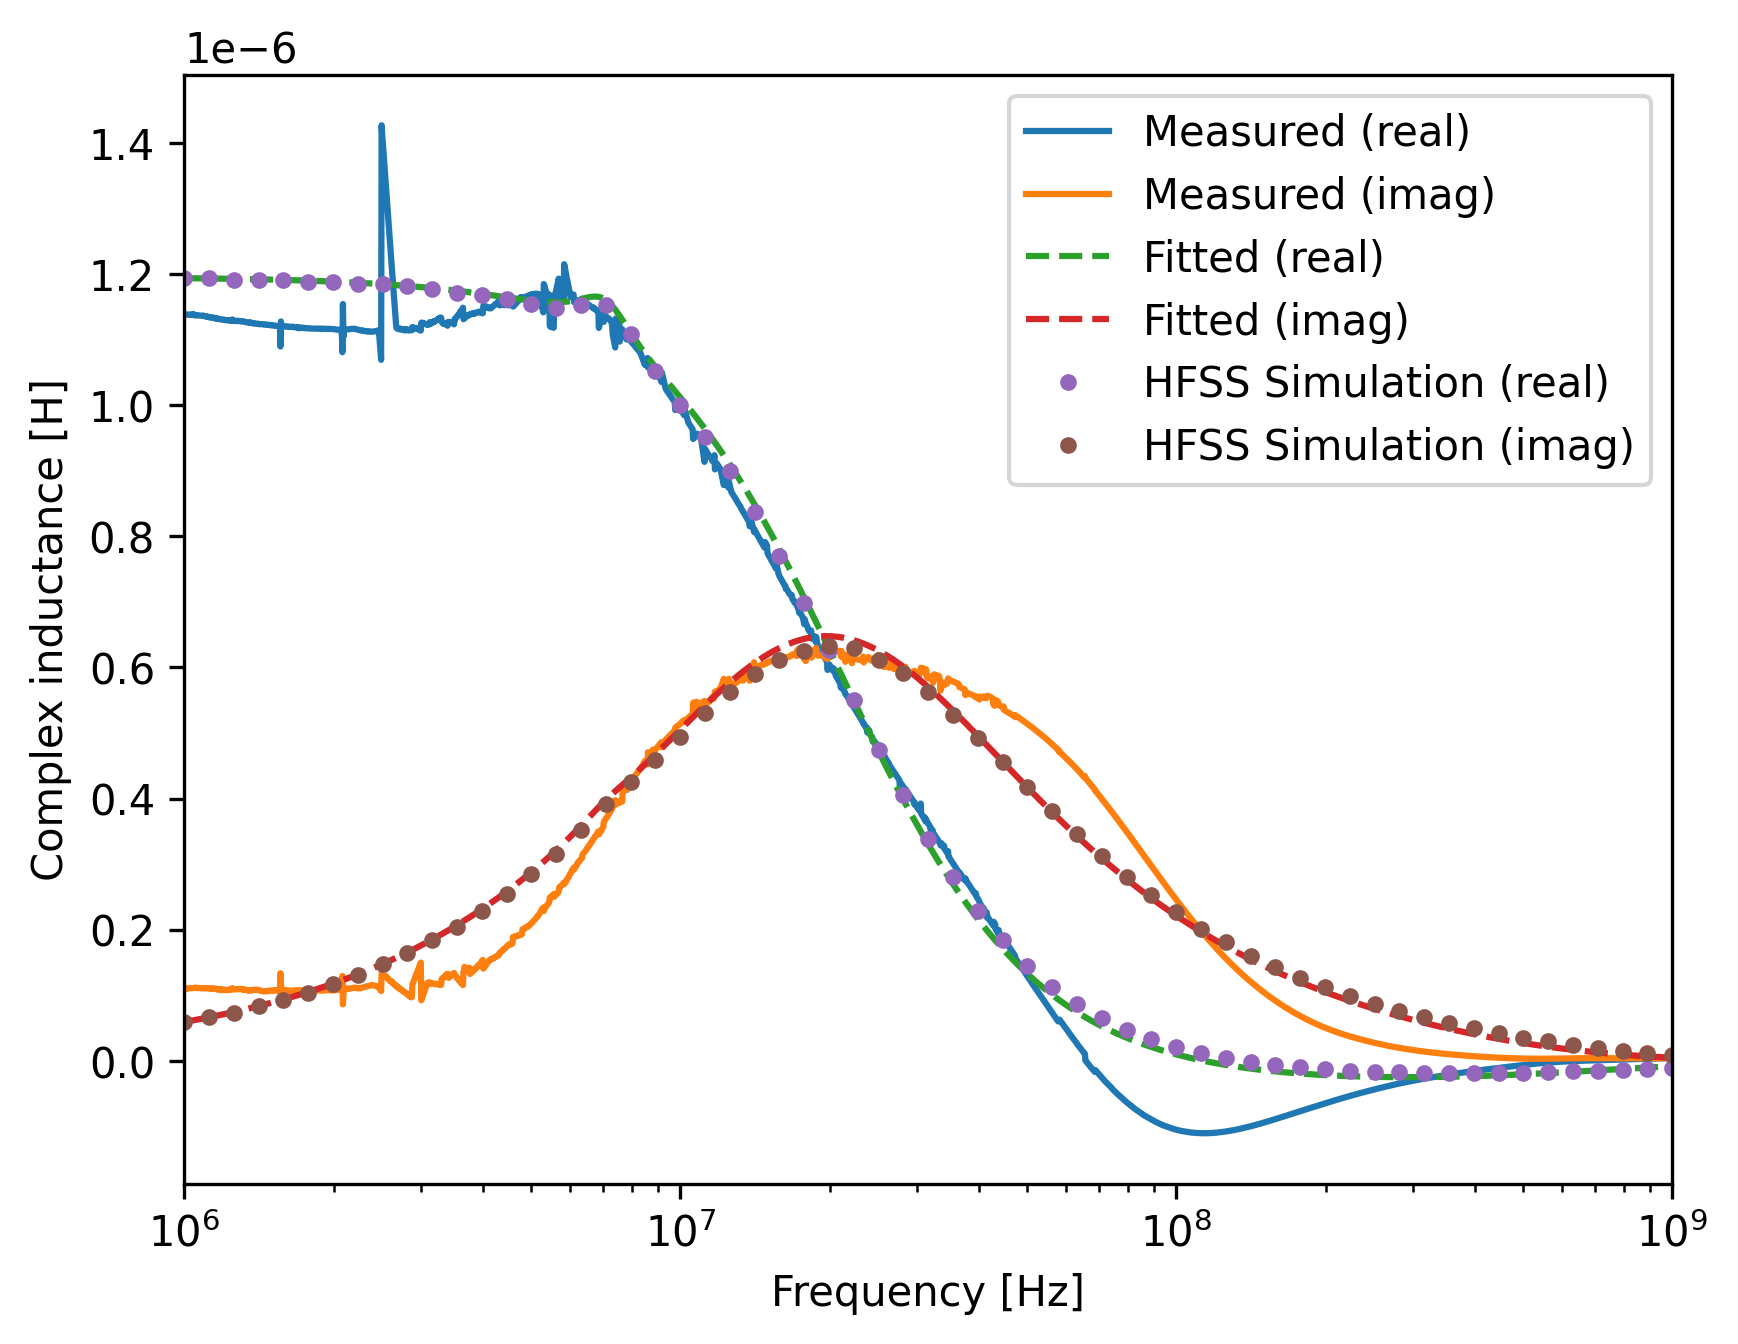
\includegraphics[width=0.45\textwidth]{inductance-measurements-and-fitting}
	}
	\subfloat[Caption of second figure]{
		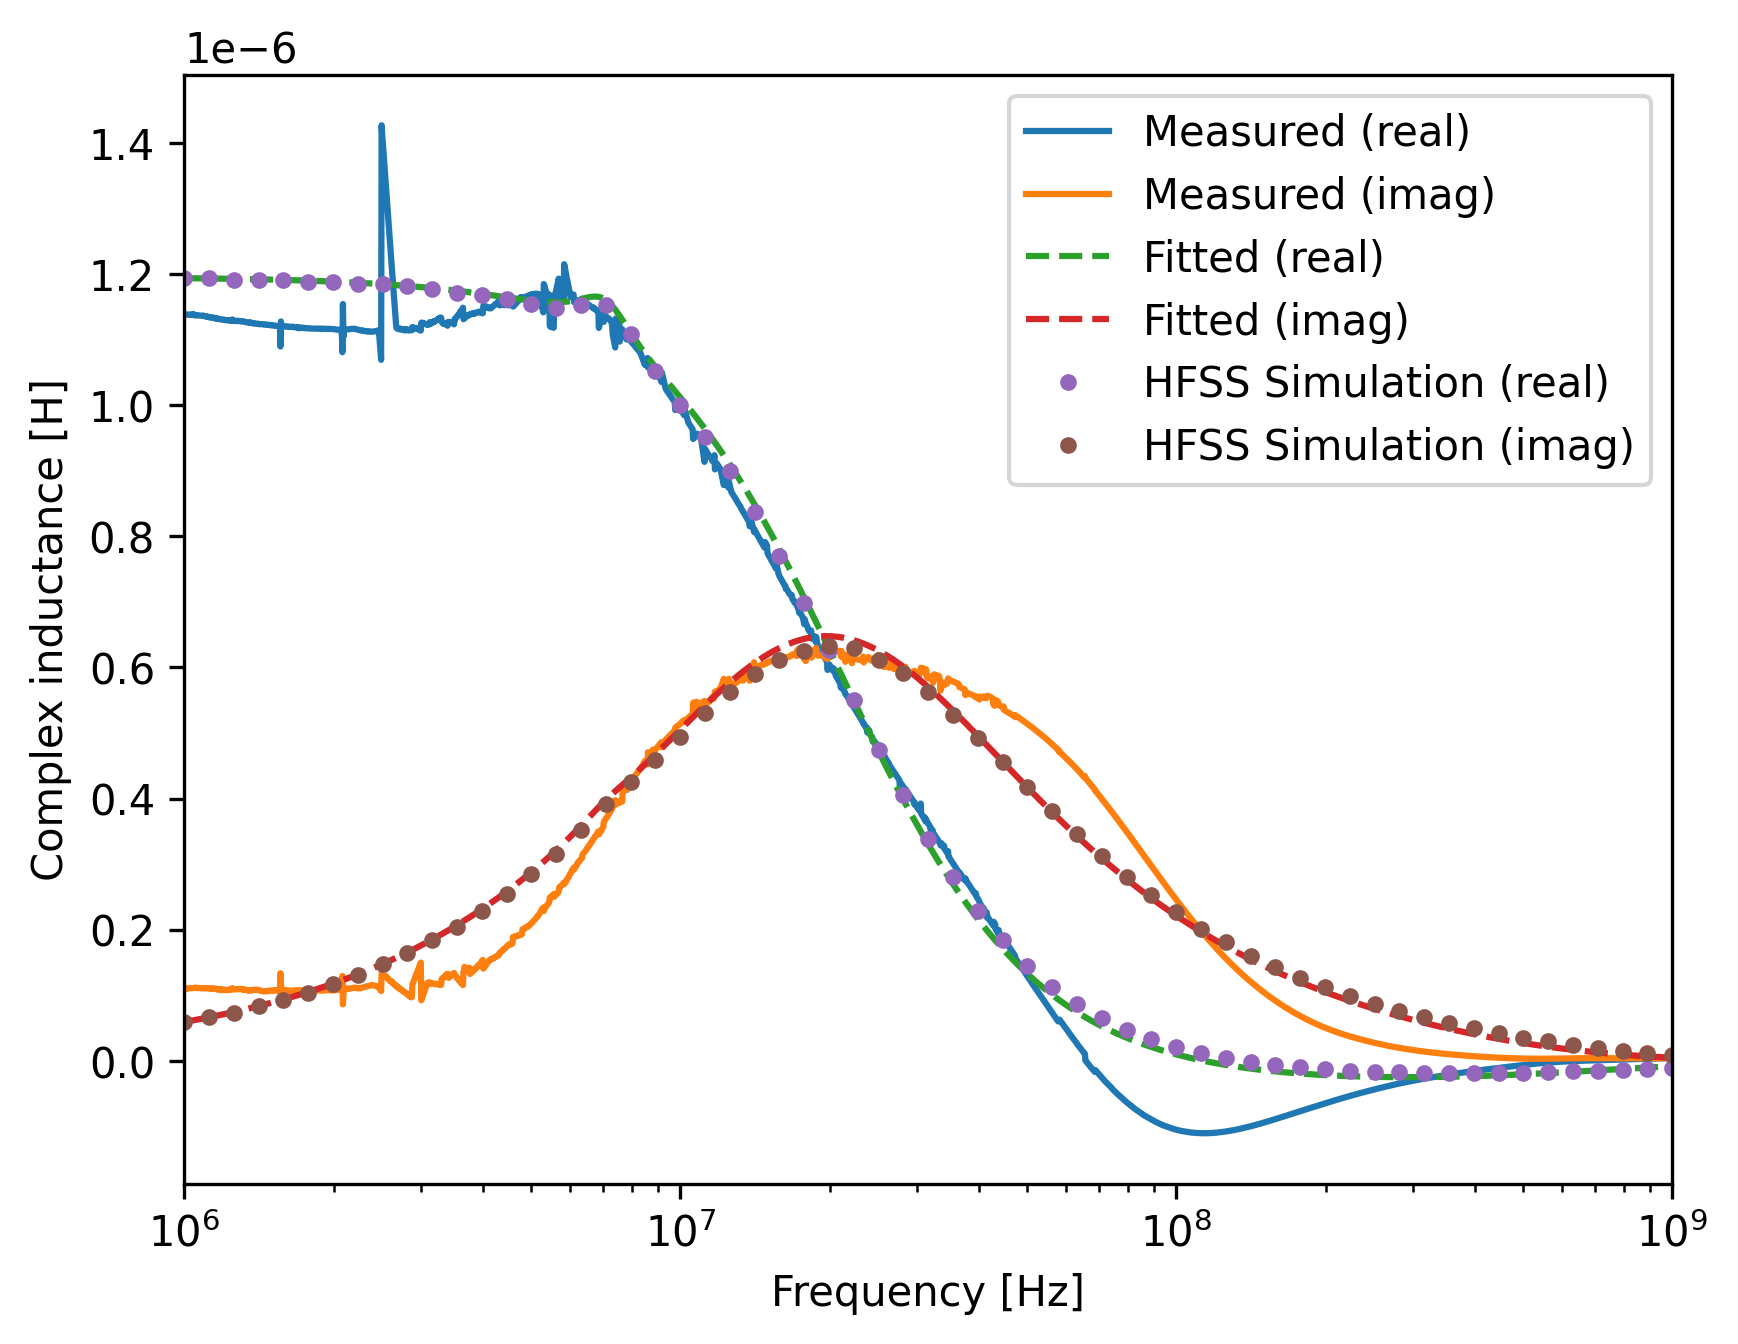
\includegraphics[width=0.45\textwidth]{inductance-measurements-and-fitting}
	}
	\caption{Example of figure}
	\label{fig:inductance-measurement}
\end{figure*}

\subsection{Experimental setup} \label{sec:experimental-setup}
In Ohm's law,
\begin{equation}
	V = R I \label{eq:ohms-law}
\end{equation}

Text can include references to figures \autoref{fig:inductance-measurement}, to sections \autoref{sec:introduction} and to equations \autoref{eq:ohms-law}.

\subsection{Simulations}
More complex formulas can be placed using \texttt{align} environment
\begin{align}
	\complexImpedance & = \iu\omega \complexInductance_{fit} \\
	& = \iu\omega \complexPermeability_{fit} \ln\left(\frac{r_e}{r_i}\right)\frac{h}{2\pi} \\
	& = \iu\omega (\mu_{fit}^{\prime}-\iu\mu_{fit}^{\prime\prime}) \ln\left(\frac{r_e}{r_i}\right)\frac{h}{2\pi}
\end{align}
In figure \autoref{fig:circuit-example} we show an example of a circuit written in latex.
Missing figures that are not available while writting the paper can be placed temoprarily \autoref{fig:circuit-example}

\begin{figure}[ht]
	\begin{circuitikz}[scale=1]
		\draw
		(0,2) to[vsource, l=\SI{48}{\volt}]
		(0,0) to[short, -*]
		(6,0) to[short, -o]
		(8,0)
		(0,2) to[R, l=$R_x$, -*]
		(2,2) to[short]
		(2,1) to[R, l=\SI{4}{\ohm}]
		(4,1) to[short,-*]
		(4,2)
		(2,2) to[short]
		(2,3) to[isource,l=\SI{3}{\ampere}, invert]
		(4,3) to[short,-*]
		(4,2) to[short,-*]
		(6,2) to[short, i=$i$, -o]
		(8,2) to[open, v=$v$]
		(8,0)
		(6,2) to[R,l=\SI{12}{\ohm}]
		(6,0);
	\end{circuitikz}
	\caption{This is an example of a circuit}
	\label{fig:circuit-example}
\end{figure}

\begin{figure}[ht]
	\centering
	\missingfigure{Experimental setup}
	\caption{Example of missing figure.}
	\label{fig:missing-figure}
\end{figure}